\FloatBarrier
\section{\mfourttwo}\label{app:offline}
We report in \Cref{tbl:offline:collection} the modules sizes of all \mfourt models (v1 and v2).
\begin{table}[!ht]
    \centering
    \small
    \begin{tabular}{rcccc}
    \toprule
          & {\bf $\text{\wvbert}^*$} & {\bf \mt} & {\bf T2U}  & {\bf Total} \\
    \midrule
    \cite{SeamlessM4TArXiv}\\
    \mfourtmd & 366M & 615M & 170M & 1151M \\
    \mfourtlg & 669M & 1370M & 287M & 2326M  \\
    \midrule
    \mfourttwo & 635M & 1370M & 295M  & 2300M \\
    \bottomrule
    \end{tabular}
    \caption{\#parameters of the building components used  in \mfourt models.\\
    *: includes the parameters of the length adaptor.
    }
    \label{tbl:offline:collection}
\end{table}

\subsection{T2U Latency improvement in \mfourttwo}\label{app:offline:t2u:latency}
\begin{figure}[!tbh]
    \centering
    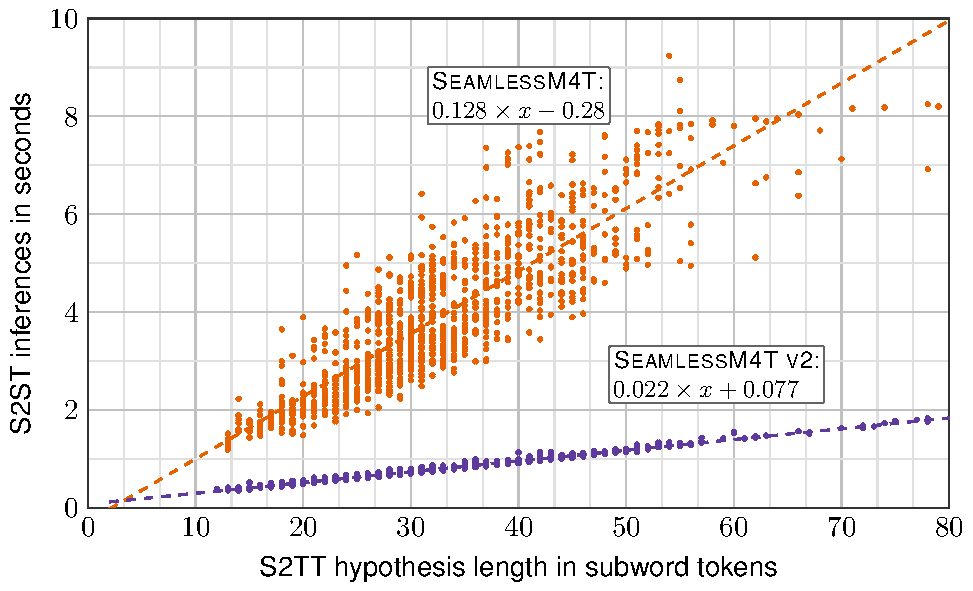
\includegraphics[width=.7\linewidth]{figures/offline/t2u_latency.pdf}
    \caption{\textbf{\sst inference time.} Comparison between \mfourt v1 and v2}
    \label{fig:offline:t2u:latency}
\end{figure}

In this section, we evaluate the latency of both \mfourtlg with the \unity architecture (autoregressive \tu), and that of \mfourtlgtwo with \unitytwo and its non-autoregressive \tu.

Each model translated 1000 audios from \fleurs~\sst test set (randomly sampled from
\texttt{hin-eng}, 
\texttt{spa-eng}, 
\texttt{por-eng},
\texttt{rus-eng},
and \texttt{eng-eng}
) while tracking input and intermediate output lengths (input audio in seconds and \st hypothesis in subword tokens) and the \sst inference time (in seconds).
Our experimental setup used 
a container with a single A100 (CUDA kernels compiled) and 96 CPUs.
We evaluated both models after warm-up with a batch-size of 1, beam search with a width of 5 for both \st and auto-regressive \tu (\mfourt), and the default decoding options (max-length, length penalties, etc.) 

The trend lines reported in \Cref{fig:offline:t2u:latency} show that
\mfourttwo is significantly faster than \mfourt v1 in \sst inference.
In fact, \tu decoding time in \mfourt scales linearly with the length of text generated with \st. On the other hand, \tu conversion time in \mfourttwo is independent from the input length. Since \tu decoding takes 70\% of the inference time in \mfourt, improving this bottleneck in \mfourttwo with NAR \tu significantly improves the total \sst inference speed by more than 3x.

\subsection{Data Statistics}

\Cref{offline:data:stats1,offline:data:stats2} provide statistics per language for data used to train \sonar speech encoders and prepare \seamlessalign per language. 
For each language we also evaluate our \sonar speech encoder  by proxy of \bleu score in the task of \fleurs~\st~\xeng using the \sonar text decoder.

We provide in \Cref{tbl:offline:s2tdata} statistics of \asr and \st data (in terms of hours of speech audio) used to train the \xt models of \mfourt. Similarly, we provide in \Cref{tbl:offline:s2stdata} statistics of \sst training data.

\newgeometry{left=.5cm, right=.5cm, bottom=4cm, top=2cm}
\begin{table}[!htb]
\scriptsize
\centering
\begin{tabular}{@{}cccccc|lrr@{}}
 \toprule
    & \multirow{2}*{\makecell{raw\\audio}} 
    & \multirow{2}*{\makecell[c]{ASR\\data}}
    & \multicolumn{3}{c|}{Automatically aligned} 
    & \multirow{2}*{\bleu} 
    & \multirow{2}*{\whisperlargeabbr}\\
    \cmidrule(lr){4-6}
    & & &  Sen2Txx & Sxx2Ten & Sxx2Sen \\
    \midrule
    Total (Hours) & 2,490,509 & 50,773 & 129,801 & 299,959 & 38,488 \\
     \midrule
    Average (support) & & & & & & 20.9 & 19.1 \\
    Average (overlap) & & & & & & \bf 22.0 & 19.1 \\
    \bottomrule
\end{tabular}\\[5pt]

    \begin{tabular}{@{}crrrrrrr@{}}
        \toprule
        \multirow{2}*{\bf code} 
        & \multirow{2}*{\makecell{\bf Raw\\\bf audio\\Hours}} 
        & \multirow{2}*{\makecell[c]{\bf ASR\\\bf data\\Hours}}
        & \multirow{2}*{\makecell[c]{\bf\sonar\\\scriptsize$\uparrow$\bleu}} 
        & \multirow{2}*{\makecell[c]{\bf\whisperlargeabbr\\\scriptsize$\uparrow$\bleu}}
        & \multicolumn{3}{c}{\textbf{Automatically aligned} (Hours)} \\[5pt]
        \cmidrule(lr){6-8}
        & & & & & Sen2Txx & Sxx2Ten & Sxx2Sen \\
        \midrule
afr  &  3,691 &  108 &  37.91 &  34.10 &  1,575 &  1,225 &  281\\
amh  &  5,676 &  51 &  11.55 &   1.90 &  874 &  2,768 &  284\\
arb  &  119,862 &  822 &  28.71 &  25.50 &  2,977 &  8,072 &  776\\
asm  &  110 &  74 &  13.27 &   5.40 &  244 &  25 &  9\\
azj  &  7,690 &  52 &  13.72 &  13.45 &  929 &  1,158 &  171\\
bel  &  61,204 &  1,104 &  15.41 &  11.70 &  1,027 &  4,434 &  366\\
ben  &  4,360 &  335 &  19.62 &  13.20 &  1,067 &  1,345 &  263\\
bos  &  2,871 &  99 &  31.25 &  29.70 &  1,017 &  661 &  112\\
bul  &  3,760 &  102 &  29.18 &  28.50 &  3,592 &  1,623 &  284\\
cat  &  49,898 &  1,738 &  35.09 &  34.20 &  1,995 &  4,411 &  354\\
ceb  &  33 &   ---  &   3.31 &   ---  &  774 &   ---  &   --- \\
ces  &  38,545 &  181 &  29.77 &  27.80 &  3,679 &  6,905 &  602\\
ckb  &   ---  &  93 &  14.56 &   ---  &  527 &   ---  &   --- \\
cmn  &  77,158 &  9,320 &  17.42 &  18.40 &  1,873 &  18,760 &  1,570\\
cym  &  16,690 &  99 &  11.66 &  13.00 &  1,167 &  4,411 &  278\\
dan  &  23,469 &  115 &  31.90 &  32.70 &  2,499 &  6,041 &  583\\
deu  &  439,595 &  3,329 &  32.72 &  34.60 &  7,478 &  17,634 &  1,921\\
ell  &  9,141 &  324 &  20.65 &  23.70 &   ---  &  2,833 &  273\\
est  &  9,013 &  131 &  24.69 &  18.70 &  1,932 &  3,346 &  607\\
fin  &  26,132 &  184 &  21.27 &  22.10 &  1,355 &  6,086 &  526\\
fra  &  233,406 &  2,057 &  31.22 &  32.20 &  9,044 &  17,380 &  3,337\\
gle  &  282 &  57 &   4.11 &   ---  &  1,121 &  121 &  32\\
glg  &  60,448 &  123 &  31.29 &  27.90 &  1,217 &  1,385 &  295\\
guj  &   ---  &  139 &  23.63 &  16.20 &  1,148 &  355 &  261\\
heb  &  34,257 &  92 &  20.71 &  21.80 &   ---  &  10,130 &  534\\
hin  &  10,583 &  150 &  19.55 &  22.00 &  1,629 &  2,977 &  530\\
hrv  &  3,857 &  304 &  28.65 &  27.00 &   ---  &  1,016 &  191\\
hun  &  22,705 &  258 &  19.86 &  21.20 &  2,351 &  4,044 &  526\\
hye  &  4,175 &  145 &  21.54 &  16.00 &  759 &  99 &  148\\
ind  &  10,109 &  269 &  25.50 &  28.95 &  1,860 &  2,658 &  510\\
isl  &  1,603 &  113 &  17.26 &   9.10 &  1,259 &  750 &  142\\
ita  &  75,285 &  588 &  25.30 &  23.60 &  5,379 &  6,508 &  817\\
jav  &  1,017 &  302 &  17.94 &   6.59 &  508 &  6 &  52\\
jpn  &  85,861 &  17,319 &  17.64 &  18.16 &  522 &  21,287 &  1,141\\
kan  &  836 &  114 &  19.39 &  11.60 &  936 &  936 &  198\\
kat  &  12,028 &  188 &  12.22 &   2.40 &  667 &  1,270 &  168\\
kaz  &  9,418 &  314 &  16.81 &   5.38 &  743 &  1,669 &  183\\
khk  &  255 &  143 &   9.02 &   0.86 &  575 &  91 &  146\\
khm  &  9,378 &  182 &  14.35 &   5.63 &  492 &   ---  &   --- \\
kir  &   ---  &  82 &  13.78 &   ---  &  684 &  99 &  58\\
kor  &  21,380 &  316 &  16.73 &  21.57 &  2,228 &  8,657 &  640\\
        \bottomrule
    \end{tabular}
     \caption{Statistics on speech encoders and amount of automatically aligned data. 
    We provide the amount of raw audio data for automatic alignment and the amount of human-provided ASR transcripts to train the speech encoders. 
    The speech encoders are evaluated for \st using BLEU on the \fleurs test set. Our model performs zero-shot \st.
    We include for reference the BLEU scores of \whisperlarge (abbreviated as \whisperlargeabbr) if the language is supported.
    Finally, the last three columns provide the amount of automatically aligned data.}\label{offline:data:stats1}
\end{table}
\begin{table}[!htb]
\scriptsize
\centering
    \begin{tabular}{@{}crrrrrrr@{}}
     \toprule
        \multirow{2}*{\bf code} 
        & \multirow{2}*{\makecell{\bf Raw\\\bf audio\\Hours}} 
        & \multirow{2}*{\makecell[c]{\bf ASR\\\bf data\\Hours}}
        & \multirow{2}*{\makecell[c]{\bf\sonar\\\scriptsize$\uparrow$\bleu}} 
        & \multirow{2}*{\makecell[c]{\bf\whisperlargeabbr\\\scriptsize$\uparrow$\bleu}}
        & \multicolumn{3}{c}{\textbf{Automatically aligned} (Hours)} \\[5pt]
        \cmidrule(lr){6-8}
         & & & & & Sen2Txx & Sxx2Ten & Sxx2Sen \\
        \midrule
lao  &  2,570 &  193 &  15.27 &  11.10 &  439 &  845 &  212\\
lit  &  2,063 &  47 &  18.50 &  14.00 &   ---  &  688 &  204\\
lug  &   ---  &  369 &  13.39 &   ---  &  197 &  186 &  203\\
lvs  &  3,295 &  53 &  25.55 &  14.30 &   ---  &  1,242 &  347\\
mal  &  3,023 &  99 &  16.10 &  16.70 &  680 &  360 &  255\\
mar  &  1,229 &  126 &  18.26 &  12.90 &  659 &  398 &  258\\
mkd  &  1,871 &  100 &  31.93 &  27.70 &  1,169 &  360 &  88\\
mlt  &  448 &  106 &  30.31 &  13.50 &  914 &  130 &  60\\
nld  &  71,089 &  1,723 &  25.52 &  24.00 &  3,965 &  6,859 &  1,210\\
nob  &  35,540 &  208 &  31.45 &  31.40 &   ---  &  7,520 &  620\\
npi  &  3,501 &  153 &  17.31 &  16.10 &  462 &  973 &  206\\
ory  &   ---  &  89 &  17.15 &   ---  &  383 &  76 &  138\\
pan  &  827 &  198 &  20.93 &  15.70 &  896 &  896 &  292\\
pbt  &  29,139 &  123 &  10.78 &   3.12 &  712 &  3,854 &  207\\
pes  &  59,072 &  386 &  22.25 &  18.96 &   ---  &  7,122 &  693\\
pol  &  50,527 &  304 &  22.01 &  22.30 &  3,002 &  9,389 &  757\\
por  &  119,965 &  269 &  35.43 &  38.10 &  4,673 &  8,696 &  928\\
ron  &  17,851 &  135 &  32.08 &  31.50 &  3,740 &  2,878 &  716\\
rus  &  105,777 &  259 &  26.53 &  27.80 &  6,603 &  13,509 &  1,252\\
slk  &  14,196 &  102 &  29.35 &  25.79 &  2,834 &  3,785 &  491\\
slv  &  4,360 &  65 &  23.72 &  17.00 &   ---  &  1,141 &  221\\
snd  &  1,748 &   ---  &   5.69 &   5.70 &  411 &  116 &  61\\
spa  &  222,235 &  1,511 &  24.31 &  23.30 &  5,025 &  17,388 &  2,727\\
srp  &  11,724 &  100 &  33.98 &  32.50 &  2,211 &  660 &  446\\
swe  &  89,271 &  144 &  33.44 &  35.30 &  2,951 &  2,951 &  840\\
swh  &  22,411 &  361 &  22.57 &   7.20 &  848 &  2,620 &  484\\
tam  &  5,464 &  245 &  15.36 &   9.20 &  730 &  1,664 &  867\\
tel  &  4,023 &  84 &  15.84 &  12.50 &  1,195 &  985 &  536\\
tgk  &  12,852 &  98 &  20.42 &  14.50 &  567 &   ---  &   --- \\
tgl  &  2,413 &  108 &  13.29 &  24.04 &  1,274 &  633 &  266\\
tha  &  14,561 &  195 &  15.43 &  15.75 &  1,357 &  3,563 &  542\\
tur  &  16,467 &  174 &  20.07 &  26.60 &  2,885 &  6,545 &  426\\
ukr  &  9,239 &  105 &  29.02 &  29.40 &  2,953 &  1,717 &  392\\
urd  &  9,623 &  185 &  17.09 &  17.20 &  763 &  3,416 &  652\\
uzn  &  5,201 &  115 &  17.54 &   6.00 &  783 &  1,846 &  157\\
vie  &  22,119 &  194 &  17.58 &  20.70 &  2,757 &  7,692 &  868\\
yor  &  11,263 &  130 &   9.93 &   1.40 &  242 &  2,653 &  425\\
yue  &   ---  &  171 &  13.09 &   ---  &  428 &   ---  &   --- \\
zlm  &  7,771 &  168 &  25.50 &  26.89 &  751 &  1,427 &  272\\
zul  &   ---  &  62 &   5.39 &   ---  &  639 &   ---  &   --- \\
       \bottomrule
    \end{tabular}
     \caption{Statistics on speech encoders and amount of automatically aligned data. 
    We provide the amount of raw audio data for automatic alignment and the amount of human-provided ASR transcripts to train the speech encoders. 
    The speech encoders are evaluated for \st using BLEU on the \fleurs test set. Our model performs zero-shot \st.
    We include for reference the BLEU scores of \whisperlarge (abbreviated as \whisperlargeabbr) if the language is supported.
    Finally, the last three columns provide the amount of automatically aligned data.}\label{offline:data:stats2}
\end{table}
\restoregeometry

\newgeometry{left=1.cm, right=1.cm, bottom=4cm, top=2cm}
\begin{table}[!htb]
\scriptsize
    \centering
    \hfill\begin{minipage}[t]{0.45\textwidth}\vspace{0pt}
    \begin{tabular}{@{}crrrrrrr@{}}
        \toprule
         & \multicolumn{3}{c}{\xeng}  
         &  \multicolumn{1}{c}{\asr}
         & \multicolumn{3}{c}{\engx} \\
        \cmidrule(lr){2-4} \cmidrule(lr){5-5} \cmidrule(lr){6-8}
         & H & P & A & H & H & P & A \\
         \midrule
        Total & 14,434 & 52,977 & 23,744 & 47,296 & 8,476 & 184,123 & 20,377 \\
        \midrule
         \toprule
         & \multicolumn{3}{c}{\xeng}  
         &  \multicolumn{1}{c}{\asr}
         & \multicolumn{3}{c}{\engx} \\
        \cmidrule(lr){2-4} \cmidrule(lr){5-5} \cmidrule(lr){6-8}
         & H & P & A & H & H & P & A \\
         \midrule
        afr & 100 & 9 & 400 & 103 & 0 & 2,218 & 400 \\
        amh & 38 & 20 & 399 & 58 & 0 & 2,218 & 400 \\
        arb & 187 & 1,035 & 394 & 1,236 & 507 & 1,352 & 400 \\
        ary & 47 & 0  & 0 & 47 & 0 & 2,218 &  \\
        arz & 47 & 0  & 0 & 47 & 0 & 2,218 &  \\
        asm & 86 & 0 & 23 & 86 & 22 & 1,987 & 203 \\
        azj & 101 & 4 & 400 & 101 & 22 & 1,987 & 400 \\
        bel & 247 & 926 & 400 & 1,172 & 22 & 1,987 &  \\
        ben & 125 & 227 & 375 & 354 & 0 & 2,218 & 400 \\
        bos & 157 &  0 & 400 & 102 & 0 & 2,218 & 400 \\
        bul & 105 & 0 & 400 & 105 & 22 & 1,987 &  \\
        cat & 445 & 1,332 & 382 & 1,833 & 506 & 1,353 & 400 \\
        ceb & 0 &  & 0 & 0 & 0 & 2,218 & 400 \\
        ces & 132 & 500 & 390 & 206 & 22 & 1,987 &  \\
        ckb & 30 & 63 & 0 & 94 & 0 & 2,218 & 400 \\
        cmn & 425 & 12,599 & 396 & 12,979 & 506 & 1,353 &  \\
        cym & 39 & 73 & 352 & 101 & 506 & 1,353 & 400 \\
        dan & 167 & 372 & 383 & 200 & 22 & 1,987 &  \\
        deu & 594 & 3,291 & 400 & 3,843 & 496 & 1,363 &  \\
        ell & 343 & 12 & 400 & 524 & 0 & 2,218 &  \\
        eng & - & - & - & 4,066 & - & - & - \\
        est & 131 & 12 & 373 & 144 & 500 & 1,359 &  \\
        eus & 217 & 61 & 0 & 279 & 0 & 2,218 & 400 \\
        fin & 154 & 477 & 368 & 209 & 22 & 1,987 & 400 \\
        fra & 574 & 2,144 & 400 & 2,429 & 22 & 2,196 &  \\
        gaz &  0  & 0     &  0  & 0     & 0 & 2,218 & 66 \\
        gle & 65 & 3 & 108 & 54 & 0 & 2,218 &  \\
        glg & 103 & 16 & 400 & 119 & 0 & 2,218 & 400 \\
        guj & 139 & 8 & 275 & 152 & 53 & 2,218 & 400 \\
        heb & 104 & 1 & 400 & 105 & 0 & 2,218 &  \\
        hin & 304 & 0 & 382 & 85 & 0 & 2,218 &  \\
        hrv & 101 & 217 & 0 & 317 & 0 & 2,218 &  \\
        hun & 308 & 446 & 400 & 288 & 22 & 1,987 &  \\
        hye & 152 & 1 & 400 & 152 & 22 & 1,987 & 400 \\
        ibo & 38 &  0 & 0 & 38 & 0 & 2,218 & 303 \\
        ind & 373 & 12 & 353 & 302 & 506 & 1,353 &  \\
        isl & 23 & 115 & 400 & 137 & 0 & 2,218 & 400 \\
        ita & 138 & 941 & 383 & 630 & 22 & 1,987 &  \\
        jav & 0 & 303 & 5 & 303 & 0 & 2,218 & 400 \\
        jpn & 514 & 19,483 & 392 & 573 & 507 & 1,352 & 400 \\
        kan & 121 & 9 & 200 & 129 & 53 & 2,218 & 400 \\
        kat & 198 & 3 & 400 & 202 & 0 & 2,218 & 400 \\
        kaz & 22 & 318 & 0 & 339 & 22 & 1,987 & 400 \\
        khk & 163 & 2 & 74 & 166 & 506 & 1,356 & 400 \\
        khm & 202 & 8 & 0 & 206 & 0 & 2,218 & 400 \\
        \bottomrule
        \end{tabular}
        \end{minipage}\hspace{15pt}\hfill
        \begin{minipage}[t]{0.45\textwidth}\vspace{0pt}
        \begin{tabular}{@{}crrrrrrr@{}}
        \toprule
         & \multicolumn{3}{c}{\xeng}  
         &  \multicolumn{1}{c}{\asr}
         & \multicolumn{3}{c}{\engx} \\
        \cmidrule(lr){2-4} \cmidrule(lr){5-5} \cmidrule(lr){6-8}
        & H & P & A & H & H & P & A \\
        \midrule
        kir & 111 & 20 & 83 & 149 & 22 & 1,987 & 400 \\
        kor & 228 & 52 & 392 & 646 & 14 & 2,218 & 400 \\
        lao & 217 &  & 400 & 217 & 0 & 2,218 & 361 \\   
        lav & 0 &  & 0 & 28 &  &  &  \\
        lit & 44 & 398 & 400 & 44 & 22 & 1,987 &  \\
        lug & 263 & 106 & 145 & 370 & 0 & 2,218 & 152 \\
        luo &  0 & 0  & 0  & 0  & 0 & 2,218 & 171 \\
        lvs & 103 & 0 & 400 & 103 & 506 & 1,353 &  \\
        mai &  0 & 0 & 0 & 0 & 0 & 2,218 & 69 \\
        mal & 59 & 55 & 313 & 114 & 0 & 2,218 & 400 \\
        mar & 100 & 25 & 312 & 110 & 22 & 1,987 & 400 \\
        mkd & 149 & 1 & 314 & 149 & 22 & 1,987 & 400 \\
        mlt & 158 & 1 & 70 & 159 & 22 & 1,987 & 400 \\
        mni & 2 & 0 & 0 & 0 & 0 & 2,218 &  \\
        mya & 150 & 8 & 0 & 157 & 0 & 2,218 &  \\
        nld & 185 & 2,037 & 386 & 1,804 & 22 & 1,987 &  \\
        \makecell[c]{nor} & 115 & 126 & 0 & 228 & 0 & 2,218 & 0 \\
        npi & 0 & 160 & 400 & 158 & 22 & 1,988 & 400 \\
        nya & 105 &  & 0 & 105 & 0 & 2,218 & 400 \\
        ory & 93 & 0 & 53 & 93 & 22 & 1,987 & 328 \\
        pan & 202 & 4 & 400 & 202 & 22 & 1,987 & 400 \\
        pbt & 152 &  & 399 & 150 & 0 & 2,218 & 400 \\
        pes & 188 & 204 & 0 & 390 & 507 & 1,352 &  \\
        pol & 88 & 725 & 386 & 377 & 22 & 1,987 &  \\
        por & 172 & 206 & 383 & 845 & 22 & 1,987 &  \\
        ron & 111 & 536 & 387 & 189 & 22 & 1,987 & 400 \\
        rus & 114 & 164 & 387 & 269 & 22 & 1,988 &  \\
        slk & 108 & 470 & 386 & 160 & 22 & 1,987 &  \\
        slv & 106 & 442 & 400 & 115 & 507 & 1,352 &  \\
        sna & 33 &  & 0 &  & 0 & 2,218 & 400 \\
        snd & 0 &  & 103 & 0 & 0 & 2,218 & 354 \\
        som & 153 &  & 0 & 152 & 0 & 2,218 & 169 \\
        spa & 385 & 1,726 & 400 & 1,886 & 22 & 2,196 &  \\
        srp & 101 & 0 & 400 & 103 & 22 & 1,987 &  \\
        swe & 116 & 19 & 0 & 122 & 505 & 1,358 &  \\
        swh & 245 & 119 & 361 & 364 & 22 & 1,987 & 400 \\
        tam & 220 & 55 & 335 & 275 & 507 & 1,352 & 400 \\
        tel & 91 & 6 & 369 & 97 & 0 & 2,218 & 400 \\
        tgk & 101 &  & 0 & 101 & 0 & 2,218 &  \\
        tgl & 191 & 0 & 373 & 103 & 0 & 2,218 & 400 \\
        tha & 133 & 72 & 387 & 269 & 0 & 2,218 & 400 \\
        tur & 241 & 39 & 362 & 380 & 506 & 1,370 &  \\
        ukr & 105 & 39 & 387 & 319 & 22 & 2,196 & 400 \\
        urd & 489 & 23 & 371 & 213 & 21 & 1,987 & 400 \\
        uzn & 155 & 16 & 344 & 171 & 22 & 1,987 & 400 \\
        vie & 247 & 32 & 349 & 216 & 53 & 2,218 &  \\
        yor & 103 & 33 & 400 & 132 & 0 & 2,218 & 201 \\
        yue & 211 & 15 & 0 & 220 & 22 & 1,987 & 400 \\
        zlm & 165 &  & 400 & 162 &  &  &  \\
        zul & 67 &  & 0 & 67 & 0 & 2,218 & 400 \\
        \bottomrule
    \end{tabular}
    \end{minipage}\hfill
\caption{\small Statistics of \asr{} and \st{} data used to train our \mfourt{} model. We list the data size in hours of speech between human-labeled (H),
pseudo-labeled ASR data (P),
and automatically aligned (A). For each language we distinguish between \engx{} for translating from English into that language, and \xeng{} for translating into English.
We qualify as high-resource, languages with more than 1000 hours of supervision. Languages with between 500 and 1000 hours are dubbed medium-resource, and languages with less than 500 hours are low-resource. If a language is not supervised during the 1+2 stages of finetuning then it is evaluated as zero-shot.
}
\label{tbl:offline:s2tdata}
\end{table}
\restoregeometry

\begin{table}[!htb]
\scriptsize
    \centering
    \vspace{-53pt}
    \hspace{-30pt}\begin{minipage}[t]{0.45\textwidth}\vspace{0pt}
    \begin{tabular}{@{}ccccc@{}}
        \toprule
        & \multicolumn{4}{c}{\bf \sst}\\\cmidrule{2-5}
         & \multicolumn{2}{c}{\xeng{}} & \multicolumn{2}{c}{\engx{}} \\
        \cmidrule(r){2-3}
        \cmidrule(l){4-5}
        {} & Primary & Automatic & Primary & Automatic \\
        \midrule
        {\bf Total} & 71,474 & 5,924 & 65,812 & 2,352 \\\midrule
        afr & 430 & 112 & 0 & 0 \\
        amh & 306 & 112 & 0 & 0 \\
        arb & 1516 & 74 & 1840 & 74 \\
        ary & 282 & 0 & 0 & 0 \\
        arz & 284 & 0 & 0 & 0 \\
        asm & 358 & 4 & 0 & 0 \\
        ast & 16 & 0 & 0 & 0 \\
        azj & 428 & 78 & 0 & 0 \\
        bel & 1462 & 112 & 0 & 0 \\
        ben & 744 & 74 & 1986 & 74 \\
        bos & 534 & 52 & 0 & 0 \\
        bul & 436 & 112 & 0 & 0 \\
        cat & 1760 & 74 & 1842 & 74 \\
        ceb & 14 & 0 & 0 & 0 \\
        ces & 912 & 74 & 1908 & 74 \\
        ckb & 390 & 0 & 0 & 0 \\
        cmn & 4970 & 74 & 1820 & 76 \\
        cym & 342 & 74 & 1842 & 70 \\
        dan & 836 & 74 & 1906 & 74 \\
        deu & 2540 & 74 & 1792 & 74 \\
        ell & 776 & 112 & 0 & 0 \\
        est & 504 & 74 & 1840 & 74 \\
        eus & 700 & 0 & 0 & 0 \\
        fin & 918 & 74 & 1904 & 74 \\
        fra & 2010 & 74 & 1794 & 76 \\
        gle & 342 & 10 & 0 & 0 \\
        glg & 458 & 110 & 0 & 0 \\
        guj & 502 & 112 & 0 & 0 \\
        hau & 392 & 0 & 0 & 0 \\
        heb & 436 & 112 & 0 & 0 \\
        hin & 678 & 74 & 1994 & 74 \\
        hrv & 1668 & 98 & 0 & 0 \\
        hun & 1032 & 110 & 0 & 0 \\
        hye & 522 & 74 & 0 & 0 \\
        ibo & 228 & 0 & 0 & 0 \\
        ind & 798 & 74 & 1838 & 74 \\
        isl & 484 & 74 & 0 & 0 \\
        ita & 1250 & 74 & 1830 & 74 \\
        jav & 694 & 6 & 0 & 0 \\
        jpn & 5664 & 74 & 1838 & 74 \\
        kan & 468 & 64 & 0 & 0 \\
        kat & 590 & 88 & 0 & 0 \\
        kaz & 778 & 78 & 0 & 0 \\
        khk & 530 & 56 & 0 & 0 \\
        khm & 602 & 0 & 0 & 0 \\
        kir & 476 & 24 & 0 & 0 \\
        kor & 666 & 74 & 2000 & 74 \\
        lao & 600 & 104 & 0 & 0 \\
        lav & 4 & 0 & 0 & 0 \\
        lin & 312 & 0 & 0 & 0 \\
        \bottomrule
    \end{tabular}
    \end{minipage}\hspace{5pt}
    \begin{minipage}[t]{0.45\textwidth}\vspace{0pt}
    \begin{tabular}{@{}ccccc@{}}
        \toprule
        & \multicolumn{4}{c}{\bf \sst}\\\cmidrule{2-5}
         & \multicolumn{2}{c}{\xeng{}} & \multicolumn{2}{c}{\engx{}} \\
        \cmidrule(r){2-3}
        \cmidrule(l){4-5}
        {} & Primary & Automatic & Primary & Automatic \\
        \midrule       
        lit & 728 & 104 & 0 & 0 \\
        ltz & 6 & 0 & 0 & 0 \\
        lug & 820 & 78 & 0 & 0 \\
        lvs & 428 & 112 & 0 & 0 \\
        mal & 412 & 108 & 0 & 0 \\
        mar & 446 & 112 & 0 & 0 \\
        mkd & 518 & 44 & 0 & 0 \\
        mlt & 528 & 18 & 1898 & 14 \\
        mni & 38 & 0 & 0 & 0 \\
        mya & 504 & 0 & 0 & 0 \\
        nld & 1848 & 74 & 1840 & 74 \\
        nno & 26 & 0 & 0 & 0 \\
        nob & 440 & 112 & 0 & 0 \\
        nor & 442 & 0 & 0 & 0 \\
        npi & 492 & 96 & 0 & 0 \\
        nya & 426 & 0 & 0 & 0 \\
        oci & 62 & 0 & 0 & 0 \\
        ory & 404 & 52 & 0 & 0 \\
        pan & 592 & 112 & 0 & 0 \\
        pbt & 488 & 182 & 0 & 0 \\
        pes & 812 & 0 & 1834 & 0 \\
        pol & 1052 & 74 & 1890 & 74 \\
        por & 752 & 74 & 1764 & 74 \\
        ron & 920 & 74 & 1898 & 74 \\
        rus & 698 & 74 & 1702 & 74 \\
        slk & 866 & 74 & 1908 & 74 \\
        slv & 844 & 110 & 0 & 0 \\
        sna & 178 & 0 & 0 & 0 \\
        snd & 0 & 28 & 0 & 0 \\
        som & 520 & 0 & 0 & 0 \\
        spa & 1760 & 74 & 1726 & 74 \\
        srp & 428 & 112 & 0 & 0 \\
        swa & 14 & 0 & 0 & 0 \\
        swe & 478 & 112 & 1840 & 0 \\
        swh & 804 & 76 & 1904 & 74 \\
        tam & 678 & 74 & 0 & 0 \\
        tel & 382 & 74 & 1990 & 74 \\
        tgk & 424 & 0 & 0 & 0 \\
        tgl & 502 & 76 & 1994 & 64 \\
        tha & 584 & 74 & 1996 & 74 \\
        tur & 676 & 74 & 1844 & 74 \\
        ukr & 506 & 74 & 1990 & 74 \\
        urd & 930 & 74 & 1896 & 74 \\
        uzn & 552 & 52 & 1906 & 54 \\
        vie & 666 & 74 & 2018 & 74 \\
        wol & 172 & 0 & 0 & 0 \\
        xho & 104 & 0 & 0 & 0 \\
        yor & 482 & 82 & 0 & 0 \\
        yue & 532 & 0 & 0 & 0 \\
        zlm & 548 & 112 & 0 & 0 \\
        zul & 320 & 0 & 0 & 0 \\
        \bottomrule
    \end{tabular}
    \end{minipage}
    \caption{\small Statistics of \sst{} data used to train our \mfourt{} model. We list the data size in hours of speech. For each language we distinguish between \textsc{Eng-X} for translating from English into that language, and \textsc{X-Eng} for translating into English.
}
\label{tbl:offline:s2stdata}
\end{table}



\subsection{Detailed results}\label{sec:offline:allresults}
In the following, we report per-language scores across all the evaluated tasks on \fleurs. Results in CSV files are shared in \url{https://github.com/facebookresearch/seamless_communication}.
\begin{itemize}
\item \fleurs~\st~\xeng: \Cref{tbl:fleurs:st:xeng:p1,tbl:fleurs:st:xeng:p2}
\item \fleurs~\st~\engx: \Cref{tbl:fleurs:st:engx:p1,tbl:fleurs:st:engx:p2}
\item \fleurs~\sst~\xeng:  \Cref{tbl:fleurs:sst:xeng:p1,tbl:fleurs:sst:xeng:p2}
\item \fleurs~\sst~\engx: \Cref{tbl:fleurs:sst:engx}
\end{itemize}

\begin{table}[htb]
\centering
\scriptsize
\begin{tabular}{@{}cccccccccc@{}}
\toprule

&\multirow{2}{*}{\whisperlargeabbr}  
&\multirow{2}{*}{\audiopalmastabbr}
& \multicolumn{2}{c}{\whisperlarge}
& \multicolumn{2}{c}{\whispermedium}
& \multicolumn{3}{c}{\mfourt}\\
&   &  
& +\makecell[c]{NLLB\\3.3B}  & +\makecell[c]{NLLB\\1.3B}
& +\makecell[c]{NLLB\\3.3B}  & +\makecell[c]{NLLB\\1.3B}
& Medium & Large-v1 & Large-v2 \\
\midrule
        afr & 34.1 & 34.7 & 34.15 & 33.66 & 29.1 & 29.77 & 38.15 & 41.04 & 42.42 \\
        amh & 1.9 & 3.8 & 0.18 & 0.16 & 0.23 & 0.04 & 14.01 & 17.11 & 21.67 \\
        arb & 25.5 & 29 & 36.47 & 34.12 & 34.35 & 32.49 & 28.22 & 32.61 & 34.6 \\
        asm & 5.4 & 9.3 & 2.07 & 2.34 & 1.14 & 0.88 & 17.4 & 18.47 & 22.29 \\
        ast & -- & 30.8 & -- & -- & -- & -- & 24.5 & 26.25 & 26.07 \\
        azj & 13.7 & 16.2 & 19.73 & 19.59 & 17.57 & 17.87 & 14.72 & 16.44 & 18.2 \\
        bel & 11.7 & 15.1 & 15.88 & 14.8 & 13.5 & 13.49 & 14.05 & 16.19 & 17.31 \\
        ben & 13.2 & 15.9 & 2.62 & 2.92 & 1.67 & 1.25 & 21.6 & 24.18 & 26.26 \\
        bos & 29.7 & 35.7 & 36.09 & 35.99 & 33.86 & 32.97 & 30.06 & 33.53 & 36.06 \\
        bul & 28.5 & 35.5 & 34.55 & 34.15 & 31.5 & 30.92 & 26.77 & 31.19 & 32.64 \\
        cat & 34.2 & 42.5 & 42.68 & 41.22 & 41.57 & 39.9 & 34.87 & 37.82 & 39.94 \\
        ceb & -- & 10.3 & -- & -- & -- & -- & 6.01 & 8.43 & 8.76 \\
        ces & 27.8 & 34.5 & 34.37 & 32.92 & 32.23 & 30.91 & 27.05 & 31.14 & 34 \\
        ckb & -- & 4 & -- & -- & -- & -- & 16.17 & 22.1 & 24.72 \\
        cmn & 18.4 & 21.3 & 25.29 & 23.6 & 25.04 & 23.24 & 17.85 & 19.94 & 22.98 \\
        cym & 13 & 7.2 & 32.19 & 30.3 & 26.77 & 25.01 & 27.36 & 31.83 & 35.12 \\
        dan & 32.7 & 37.9 & 38.38 & 37.45 & 35.85 & 34.45 & 31.92 & 33.76 & 37.23 \\
        deu & 34.6 & 38.7 & 41.28 & 41.22 & 40.25 & 39.62 & 33.39 & 35.64 & 37 \\
        ell & 23.7 & 18.8 & 31.72 & 30.82 & 28.58 & 27.75 & 23.42 & 25.93 & 27.1 \\
        est & 18.7 & 31.7 & 31.92 & 30.54 & 29.46 & 28.43 & 24.49 & 29.65 & 31.55 \\
        fin & 22.1 & 29.3 & 32.71 & 30.71 & 31.63 & 29.19 & 23.05 & 26.61 & 27.95 \\
        fra & 32.2 & 36.5 & 40.06 & 39.23 & 38.92 & 37.94 & 30.69 & 32.96 & 33.97 \\
        ful & -- & 0.29 & -- & -- & -- & -- & 0.62 & 0.81 & 0.89 \\
        gaz & -- & 0.3 & -- & -- & -- & -- & 0.23 & 0.47 & 0.45 \\
        gle & -- & 0.3 & -- & -- & -- & -- & 10.05 & 10.69 & 15.32 \\
        glg & 27.9 & 34.7 & 35.78 & 35.19 & 33.89 & 33.42 & 29.47 & 32.53 & 34.55 \\
        guj & 16.2 & 12.2 & 9.3 & 9.27 & 6.56 & 6.39 & 25.47 & 28.33 & 31.43 \\
        hau & 0.4 & 0.6 & 2.67 & 2.41 & 2.37 & 2.62 & 0.49 & 0.44 & 0.69 \\
        heb & 21.8 & 0.4 & 31.14 & 29.48 & 27.33 & 26.4 & 24.66 & 28.8 & 32.23 \\
        hin & 22 & 21.7 & 27.82 & 26.69 & 24.64 & 23.09 & 23.51 & 26.59 & 28.21 \\
        hrv & 27 & 30.6 & 32.7 & 31.99 & 30.37 & 29.79 & 26.78 & 29.92 & 30.79 \\
        hun & 21.2 & 29.2 & 30.16 & 27.9 & 27.69 & 25.86 & 18.32 & 24.23 & 27.78 \\
        hye & 16 & 10.2 & 21.27 & 20.19 & 15.35 & 14.02 & 24.93 & 27.86 & 31.73 \\
        ibo & -- & 0.3 & -- & -- & -- & -- & 0.72 & 1.28 & 2.68 \\
        ind & 29.1 & 34.2 & 38.48 & 37.65 & 37.05 & 35.92 & 26.74 & 29.35 & 32.71 \\
        isl & 9.1 & 17.8 & 19.11 & 18.14 & 14.18 & 15.23 & 19.31 & 23.75 & 26.73 \\
        ita & 23.6 & 27.8 & 30.14 & 30.2 & 30.01 & 29.84 & 22.53 & 25.38 & 26.5 \\
        jav & 6.2 & 9.7 & 12.42 & 11.97 & 11.66 & 10.56 & 18.56 & 20.25 & 23.35 \\
        jpn & 18.9 & 11.1 & 25.35 & 24.11 & 23.89 & 23.07 & 12.74 & 15.71 & 18.23 \\
        kam & -- & 1.6 & -- & -- & -- & -- & 1.97 & 2.61 & 2.8 \\
        kan & 11.6 & 4.8 & 16.17 & 15.24 & 2.09 & 2.3 & 21.01 & 23.29 & 25.05 \\
        kat & 2.4 & 13.6 & 0.27 & 0.23 & 0.06 & 0.06 & 15.94 & 18.95 & 21.71 \\
        kaz & 5.4 & 9.5 & 19.5 & 19.23 & 15.34 & 15.5 & 20.59 & 21.6 & 24.28 \\
        kea & -- & 29.4 & -- & -- & -- & -- & 22.79 & 27.61 & 29.96 \\
        khk & 1 & 10.1 & 0.21 & 0.17 & 0.45 & 0.45 & 12.96 & 16.47 & 19.56 \\
        khm & 6.1 & 0.1 & 0.7 & 0.72 & 0.05 & 0.02 & 15.91 & 18.93 & 22.3 \\
        kir & -- & 8.61 & -- & -- & -- & -- & 15.66 & 17.45 & 19.62 \\
        kor & 21.3 & 19.4 & 27.41 & 26.01 & 26.95 & 25.32 & 17.26 & 19.17 & 24.11 \\
        lao & 11 & 9.5 & 12 & 10.87 & 10.11 & 8.43 & 17.11 & 20.18 & 24.99 \\
        lin & 1 & 0.7 & 6.02 & 5.67 & 4.34 & 4.61 & 0.72 & 1.07 & 1.3 \\
        \bottomrule
    \end{tabular}
        \caption{\textbf{\fleurs-\st~\xeng results.} We report \bleu scores as described in \Cref{tab:metrics}. (part 1/2)}\label{tbl:fleurs:st:xeng:p1}
\end{table}


\begin{table}[htb]
\centering
\scriptsize
\begin{tabular}{@{}cccccccccc@{}}
\toprule
\multirow{2}{*}{Model}
&\multirow{2}{*}{\whisperlargeabbr}  
&\multirow{2}{*}{\audiopalmastabbr}
& \multicolumn{2}{c}{\whisperlarge}
& \multicolumn{2}{c}{\whispermedium}
& \multicolumn{3}{c}{\mfourt}\\
&   &  
& +\makecell[c]{NLLB\\3.3B}  & +\makecell[c]{NLLB\\1.3B}
& +\makecell[c]{NLLB\\3.3B}  & +\makecell[c]{NLLB\\1.3B}
& Medium & Large-v1 & Large-v2 \\
\midrule
        lit & 14 & 26.8 & 24.45 & 23.42 & 21.12 & 19.83 & 16.71 & 21.59 & 24.12 \\
        ltz & 16.8 & 16.1 & 13.7 & 12.64 & 9.98 & 9.14 & 10.75 & 14.41 & 16.75 \\
        lug & -- & 1.6 & -- & -- & -- & -- & 14.58 & 16.86 & 18.41 \\
        luo & -- & 0.6 & -- & -- & -- & -- & 0.54 & 0.73 & 0.95 \\
        lvs & 14.3 & 30.5 & 29.36 & 28.27 & 27.06 & 26.35 & 23.4 & 27.85 & 30.37 \\
        mal & 16.7 & 12.2 & 3.57 & 3.45 & 2.47 & 2.29 & 17 & 21.77 & 25.96 \\
        mar & 12.9 & 17.1 & 15.44 & 15.26 & 11.14 & 11.21 & 19.26 & 22.36 & 27.42 \\
        mkd & 27.7 & 30.8 & 37.25 & 35.79 & 35.13 & 33.54 & 30.03 & 34.58 & 35.54 \\
        mlt & 13.5 & 12.4 & 16.96 & 15.94 & 12.5 & 12.05 & 34.6 & 38.63 & 40.39 \\
        mri & 10.2 & 1.2 & 13.08 & 12.2 & 6.25 & 5.84 & 0.67 & 1.09 & 1.28 \\
        mya & 0.4 & 0 & 0.29 & 0.33 & 0.14 & 0.18 & 12.86 & 15.54 & 17.77 \\
        nld & 24 & 29.1 & 31.28 & 30.39 & 30.08 & 28.94 & 23.14 & 27.18 & 27.8 \\
        nob & 31.4 & 34.6 & 37.43 & 35.55 & 36.22 & 33.67 & 30.87 & 33.96 & 34.78 \\
        npi & 16.1 & 16.2 & 15.18 & 14.71 & 11.46 & 10.76 & 21.3 & 24.76 & 29.18 \\
        nso & -- & 1.1 & -- & -- & -- & -- & 1.64 & 2.04 & 2.8 \\
        nya & -- & 1.4 & -- & -- & -- & -- & 15.87 & 17.3 & 19.41 \\
        oci & 20.2 & 22.9 & 22.39 & 21.27 & 18.91 & 18.17 & 14.36 & 18.74 & 22.74 \\
        ory & -- & 8.9 & -- & -- & -- & -- & 19.14 & 22.61 & 26.59 \\
        pan & 15.7 & 6 & 8.22 & 9.8 & 5.37 & 6.09 & 21.77 & 24.36 & 28.05 \\
        pbt & 3.4 & 0.4 & 2.78 & 3.47 & 1.03 & 0.72 & 7.17 & 12.21 & 17.19 \\
        pes & 19.6 & 25.7 & 29.41 & 27.71 & 25.24 & 23.34 & 23.62 & 28.22 & 30.27 \\
        pol & 22.3 & 25.3 & 28.36 & 27.58 & 27.69 & 26.84 & 18.58 & 22.3 & 24.41 \\
        por & 38.1 & 38.4 & 45.47 & 43.97 & 44.67 & 43.07 & 34.12 & 38.41 & 38.4 \\
        ron & 31.5 & 35.7 & 38.32 & 37.6 & 36.16 & 35.07 & 28.96 & 32.67 & 35.03 \\
        rus & 27.8 & 31.2 & 34.37 & 32.66 & 33.8 & 32.34 & 23.68 & 28.33 & 30.17 \\
        slk & 26.1 & 32.3 & 35.52 & 34.42 & 34.3 & 32.45 & 26.49 & 31.5 & 32.6 \\
        slv & 17 & 27.4 & 26.93 & 25.74 & 23.83 & 22.32 & 18.83 & 24.62 & 26.29 \\
        sna & 1.8 & 0.4 & 4.17 & 4.2 & 0.07 & 0.02 & 2.13 & 2.86 & 3.17 \\
        snd & 5.7 & 1.4 & 4.65 & 4.92 & 2.35 & 2.44 & 6.15 & 7.54 & 9.69 \\
        som & 0.7 & 0.9 & 0.55 & 0.64 & 0.54 & 0.37 & 12.67 & 15.51 & 17.91 \\
        spa & 23.3 & 26.9 & 30.45 & 29.44 & 29.14 & 28.29 & 21.53 & 25.06 & 25.49 \\
        srp & 32.5 & 34.3 & 39.24 & 37.42 & 36.52 & 35.24 & 31.33 & 35.43 & 37.67 \\
        swe & 35.3 & 40.4 & 41.24 & 39.65 & 39.87 & 38.88 & 31.49 & 34.6 & 36.89 \\
        swh & 7.2 & 9.1 & 23.38 & 22.83 & 18.8 & 18.05 & 23.18 & 26.16 & 31.14 \\
        tam & 9.2 & 15 & 19.65 & 18.15 & 15.39 & 14.43 & 12.08 & 15.87 & 22.17 \\
        tel & 12.5 & 13.3 & 2.76 & 2.29 & 1.48 & 1.25 & 20.74 & 22.32 & 25.14 \\
        tgk & 14.5 & 17.1 & 6.07 & 7.47 & 11.42 & 11.38 & 23.08 & 26.67 & 28.3 \\
        tgl & 24.4 & 15.6 & 36.93 & 35.38 & 34.76 & 33.75 & 19.76 & 23.5 & 26.35 \\
        tha & 16.1 & 15 & 21.47 & 20.15 & 18.58 & 17.37 & 15.04 & 18.94 & 23.22 \\
        tur & 26.6 & 30.1 & 35.84 & 33.58 & 34.8 & 32.91 & 22.54 & 25.81 & 30.74 \\
        ukr & 29.4 & 26.9 & 36.35 & 36.04 & 35.14 & 34.85 & 26.46 & 30.47 & 32.86 \\
        umb & -- & 0.9 & -- & -- & -- & -- & 0.39 & 0.83 & 0.97 \\
        urd & 17.2 & 13.3 & 25.82 & 25.06 & 21.86 & 21 & 20.09 & 22.82 & 24.41 \\
        uzn & 6 & 17.2 & 6.6 & 6.73 & 4.02 & 4.23 & 16.92 & 22.24 & 25.68 \\
        vie & 20.4 & 15.6 & 27.26 & 25.88 & 25.28 & 23.48 & 18.68 & 21.43 & 26 \\
        wol & -- & 0.3 & -- & -- & -- & -- & 0.97 & 1.21 & 1.67 \\
        xho & -- & 0.2 & -- & -- & -- & -- & 3.25 & 3.98 & 7.2 \\
        yor & 1.4 & 0.7 & 3.2 & 3.01 & 1.02 & 1.11 & 12.05 & 13.71 & 14.66 \\
        yue & -- & 7.4 & -- & -- & -- & -- & 8.14 & 13.16 & 19.04 \\
        zlm & 27.3 & 31.9 & 34.93 & 34.17 & 33.22 & 32.8 & 26.37 & 29.97 & 30.96 \\
        zul & -- & 1.9 & -- & -- & -- & -- & 3.68 & 6.4 & 10.38 \\
        \bottomrule
    \end{tabular}
    \caption{\textbf{\fleurs-\st~\xeng results.} We report \bleu scores as described in \Cref{tab:metrics}. (part 2/2)}\label{tbl:fleurs:st:xeng:p2}
\end{table}

\begin{table}[htb]
\centering
\scriptsize
\begin{tabular}{@{}cccccccc@{}}
\toprule
& \multicolumn{2}{c}{\whisperlarge}
& \multicolumn{2}{c}{\whispermedium}
& \multicolumn{3}{c}{\mfourt}\\ 
& +\makecell[c]{NLLB\\3.3B}  & +\makecell[c]{NLLB\\1.3B}
& +\makecell[c]{NLLB\\3.3B}  & +\makecell[c]{NLLB\\1.3B}
& Medium & Large-v1 & Large-v2 \\
\midrule
amh & 12.11 & 11.37 & 12.25 & 11.52 & 10.01 & 11.9 & 12.19 \\
arb & 24.3 & 23.12 & 24.36 & 23.04 & 19.95 & 22.86 & 23.27 \\
asm & 6.51 & 6.77 & 6.35 & 6.16 & 5.98 & 7.1 & 6.95 \\
ast & 23.92 & 22.82 & 23.66 & 22.16 & -- & -- & -- \\
azj & 11.54 & 11.48 & 11.51 & 10.68 & 9.17 & 10.55 & 11.08 \\
bel & 12.17 & 11.34 & 11.93 & 10.96 & 8.58 & 10.29 & 11.18 \\
ben & 15.02 & 14.62 & 14.95 & 14.29 & 13.21 & 14.93 & 15.1 \\
bos & 27.52 & 26.11 & 26.91 & 25.39 & 24.25 & 27.1 & 27.67 \\
bul & 37.03 & 35.74 & 36.87 & 34.87 & 30.39 & 35.49 & 36.63 \\
cat & 36.17 & 34.85 & 35.33 & 34 & 32.65 & 35.64 & 36.43 \\
ceb & 24.59 & 23.17 & 23.6 & 22.62 & 21.62 & 22.37 & 23.42 \\
ces & 27.82 & 26.8 & 27.47 & 26.32 & 22.59 & 25.18 & 26.34 \\
ckb & 9.88 & 8.49 & 8.98 & 8.22 & 8.21 & 10.29 & 9.63 \\
cmn & 29.65 & 29.18 & 29.01 & 28.76 & 25.79 & 29.55 & 29.81 \\
cym & 38.3 & 34.05 & 37.05 & 32.95 & 33.71 & 37.61 & 38.46 \\
dan & 38.03 & 36.91 & 37.61 & 36.16 & 34.72 & 39.21 & 39.39 \\
deu & 34.94 & 33.07 & 33.68 & 32.2 & 28.57 & 32.24 & 32.81 \\
ell & 22.97 & 22.13 & 22.33 & 21.52 & 19.35 & 22.17 & 22.68 \\
est & 22.26 & 19.63 & 21.78 & 19.55 & 17.63 & 22.05 & 22.39 \\
fin & 20.65 & 18.98 & 20.3 & 18.4 & 15.75 & 20.37 & 20.3 \\
fra & 43.48 & 42.53 & 42.12 & 41.18 & 37.39 & 41.41 & 42.18 \\
ful & 2.19 & 1.25 & 2.03 & 1.27 & 0.74 & 0.99 & 0.43 \\
gaz & 2.1 & 1.84 & 3.37 & 1.74 & 2.81 & 5.51 & 4.83 \\
gle & 24.64 & 22.48 & 24 & 22.28 & 20.7 & 23.25 & 24.41 \\
glg & 30.5 & 29.78 & 29.98 & 28.86 & 27.12 & 28.94 & 29.53 \\
guj & 19.79 & 18.72 & 19.44 & 18.19 & 17.71 & 20 & 20.57 \\
hau & 21.76 & 20.27 & 20.69 & 19.36 & -- & -- & -- \\
heb & 26.43 & 23.58 & 25.13 & 23.03 & 19.64 & 25.09 & 25.93 \\
hin & 30.2 & 29.36 & 29.23 & 28.15 & 27.11 & 29.28 & 29.01 \\
hrv & 25.02 & 23.66 & 24.14 & 22.59 & 20.98 & 23.2 & 24.17 \\
hun & 22.73 & 20.41 & 22.31 & 20.18 & 16.72 & 20.21 & 21.32 \\
hye & 17.5 & 14.64 & 17.62 & 15.01 & 14.81 & 16.7 & 16.79 \\
ibo & 14.33 & 13.45 & 13.91 & 12.89 & 13.57 & 13.92 & 14.23 \\
ind & 38.81 & 38.48 & 37.39 & 37 & 33.73 & 36.46 & 36.67 \\
isl & 20.42 & 16.95 & 21.42 & 16.96 & 15.55 & 21.29 & 20.58 \\
ita & 25.97 & 25.19 & 25.06 & 24.04 & 21.87 & 23.92 & 24.32 \\
jav & 21.81 & 20.97 & 20.57 & 19.67 & 19.77 & 20.62 & 21.14 \\
jpn & 35.95 & 32.87 & 35.3 & 32.7 & 31.87 & 34.96 & 35.24 \\
kam & 2.03 & 2.9 & 2.03 & 2.96 & -- & -- & -- \\
kan & 17.31 & 16.08 & 16.48 & 15.62 & 13.45 & 15.18 & 15.63 \\
kat & 12.53 & 11.53 & 12.32 & 10.8 & 9.82 & 12.12 & 12.28 \\
kaz & 18.46 & 16.65 & 18.12 & 16.43 & 15.48 & 18.89 & 19.1 \\
kea & 19.49 & 16.77 & 19.26 & 17 & -- & -- & -- \\
khk & 11.22 & 9.86 & 11.25 & 9.93 & 9.77 & 12.25 & 12.36 \\
khm & 0.53 & 0.56 & 0.56 & 0.49 & 0.66 & 0.36 & 0.55 \\
kir & 10.29 & 10.6 & 10.19 & 10.34 & 9.8 & 11.5 & 11.8 \\
kor & 10.41 & 8.75 & 10.55 & 8.59 & 10.39 & 11.4 & 12.82 \\
lao & 54.34 & 53.61 & 54.68 & 53.41 & 54.49 & 55.19 & 55.66 \\
lin & 13.54 & 13.44 & 13.49 & 13.46 & -- & -- & -- \\
\bottomrule
\end{tabular}
\caption{\textbf{\fleurs-\st~\engx results.} We report \bleu scores as described in \Cref{tab:metrics}. (part 1/2)}\label{tbl:fleurs:st:engx:p1}
\end{table}


\begin{table}[htb]
\centering
\scriptsize
\begin{tabular}{@{}cccccccc@{}}
\toprule
& \multicolumn{2}{c}{\whisperlarge}
& \multicolumn{2}{c}{\whispermedium}
& \multicolumn{3}{c}{\mfourt}\\ 
& +\makecell[c]{NLLB\\3.3B}  & +\makecell[c]{NLLB\\1.3B}
& +\makecell[c]{NLLB\\3.3B}  & +\makecell[c]{NLLB\\1.3B}
& Medium & Large-v1 & Large-v2 \\
\midrule
lit & 21.54 & 19.6 & 21.57 & 19.09 & 16.09 & 20.45 & 19.82 \\
ltz & 22.85 & 21.06 & 22.82 & 20.4 & -- & -- & -- \\
lug & 6.96 & 6.16 & 7 & 6 & 6.4 & 6.85 & 6.85 \\
luo & 9.41 & 9.58 & 9.2 & 9.66 & 9.59 & 9.66 & 9.63 \\
lvs & 22.55 & 19.01 & 22.08 & 18.69 & 20.09 & 24.34 & 25.13 \\
mal & 12.44 & 11.94 & 12.3 & 11.5 & 11 & 13.87 & 13.1 \\
mar & 14 & 12.6 & 13.48 & 12.68 & 11.36 & 13.15 & 13.86 \\
mkd & 29.89 & 27.66 & 29.62 & 26.97 & 26.53 & 28.87 & 30.46 \\
mlt & 24.74 & 22.43 & 24.07 & 22.4 & 24.03 & 27.2 & 28.28 \\
mri & 17.89 & 18.8 & 17.24 & 18.16 & -- & -- & -- \\
mya & 39.58 & 41.13 & 41.22 & 41.8 & 41.47 & 42.52 & 45.14 \\
nld & 25.59 & 24.14 & 24.78 & 23.8 & 21.68 & 23.82 & 24.08 \\
nob & 28.93 & 28.84 & 28.44 & 28.45 & 26.84 & 28.96 & 29.03 \\
npi & 13.47 & 13.01 & 14.5 & 13.24 & 15.3 & 16.49 & 16.44 \\
nso & 19.52 & 19.27 & 19.3 & 19.03 & -- & -- & -- \\
nya & 10.95 & 10.96 & 10.71 & 10.92 & 10.38 & 11.06 & 11.88 \\
oci & 30.1 & 29.34 & 29.25 & 28.41 & -- & -- & -- \\
ory & 13.4 & 13.83 & 13.34 & 13.35 & 12.59 & 13.75 & 14.01 \\
pan & 22.83 & 21.59 & 22 & 21.21 & 19.53 & 22.09 & 21.71 \\
pbt & 12.75 & 11.52 & 12.85 & 12.02 & 11.14 & 12.01 & 11.71 \\
pes & 21.97 & 21.06 & 21.53 & 20.78 & 18.32 & 20.62 & 21.83 \\
pol & 18.26 & 16.87 & 17.97 & 16.29 & 14.59 & 17 & 18.49 \\
por & 43 & 41.66 & 41.13 & 40.36 & 38.01 & 40.56 & 42.33 \\
ron & 31.68 & 30.56 & 31.24 & 29.91 & 29.32 & 31.98 & 33.62 \\
rus & 27.97 & 26.74 & 26.98 & 26.31 & 22.08 & 25.91 & 26.05 \\
slk & 28.87 & 26.81 & 28.52 & 25.87 & 22.64 & 27.12 & 28.17 \\
slv & 24.88 & 22.56 & 24.6 & 22.02 & 19.37 & 23.23 & 23.58 \\
sna & 7.59 & 7.5 & 7.05 & 7.01 & 5.8 & 6.88 & 7.78 \\
snd & 20.11 & 19.39 & 20.1 & 19.05 & 18.89 & 19.51 & 19.91 \\
som & 9.96 & 10.31 & 10.12 & 10.06 & 8.5 & 9.98 & 9.91 \\
spa & 25.75 & 25.7 & 25.06 & 25.07 & 21.14 & 23.9 & 23.44 \\
srp & 31.07 & 28.24 & 30.29 & 27.42 & 26.77 & 29.95 & 31.12 \\
swe & 38.94 & 36.99 & 38.35 & 36.21 & 34 & 38.41 & 39.32 \\
swh & 28.72 & 27.54 & 27.21 & 26.44 & 26.16 & 28.64 & 28.74 \\
tam & 15.81 & 15.46 & 15.7 & 15.2 & 13.28 & 15.54 & 15.85 \\
tel & 20.59 & 18.9 & 20.45 & 18.48 & 17.43 & 19.57 & 20.02 \\
tgk & 19.49 & 17.96 & 19.25 & 17.85 & 16.59 & 18.91 & 19.3 \\
tgl & 28.87 & 27.87 & 27.76 & 26.66 & 26.1 & 28.34 & 28.82 \\
tha & 51.02 & 48.18 & 51.13 & 48.64 & 49.8 & 50.91 & 52.37 \\
tur & 23.6 & 21.49 & 23.2 & 21.28 & 19.36 & 22.26 & 22.97 \\
ukr & 25.63 & 22.86 & 25.25 & 22.54 & 20.75 & 24.39 & 24.85 \\
umb & 0.84 & 1.21 & 0.79 & 1.22 & -- & -- & -- \\
urd & 21.58 & 20.95 & 21.56 & 20.88 & 18.86 & 20.62 & 20.98 \\
uzn & 15.83 & 13.62 & 15.3 & 13.25 & 12.83 & 14.6 & 14.44 \\
vie & 37.06 & 36.29 & 36.13 & 35.78 & 32.66 & 35.36 & 36.04 \\
wol & 5.16 & 4.35 & 5.26 & 4.43 & -- & -- & -- \\
xho & 10.84 & 10.78 & 10.68 & 10.24 & -- & -- & -- \\
yor & 3.47 & 3.62 & 3.35 & 3.8 & 4.44 & 4.49 & 4.4 \\
yue & 0.25 & 0.66 & 0.27 & 0.62 & 0.23 & 0.43 & 0.24 \\
zlm & 35.18 & 34.23 & 34.02 & 32.73 & 21.45 & 34.14 & 29.72 \\
zul & 14.3 & 13.49 & 13.36 & 12.64 & 11.86 & 13.52 & 13.57 \\
\bottomrule
\end{tabular}
\caption{\textbf{\fleurs-\st~\engx results.} We report \bleu scores as described in \Cref{tab:metrics}. (part 2/2)}\label{tbl:fleurs:st:engx:p2}
\end{table}

\begin{table}[htb]
\centering
\scriptsize
\begin{tabular}{@{}ccccccccc@{}}
\toprule
& \multicolumn{2}{c}{\whisperlarge}
& \multicolumn{2}{c}{\whispermedium}
& \multicolumn{1}{c}{\makecell[c]{\textsc{Whisper}}}
& \multicolumn{3}{c}{\mfourt}\\ 
& +\makecell[c]{NLLB\\3.3B}  & +\makecell[c]{NLLB\\1.3B}
& +\makecell[c]{NLLB\\3.3B}  & +\makecell[c]{NLLB\\1.3B}
& \makecell[c]{\textsc{Large-v2}\\\st}
& Medium & Large-v1 & Large-v2 \\
\cmidrule(lr){2-6}
& \multicolumn{5}{c}{+ \yourtts }\\
        \midrule
        afr & 34.46 & 33.72 & 30.59 & 30.64 & 34.83 & 44.92 & 39.74 & 51.37 \\
        amh & 0.36 & 0.39 & 0.43 & 0.28 & 1.66 & 18.72 & 13.88 & 24.86 \\
        arb & 38.37 & 35.97 & 35.49 & 34.12 & 25.38 & 34.14 & 26.47 & 37.73 \\
        asm & 2.03 & 2.19 & 1.04 & 0.98 & 5.12 & 18.78 & 16.66 & 24.45 \\
        ast & -- & -- & -- & -- & -- & 27.85 & 22.97 & 30.62 \\
        azj & 20.42 & 19.98 & 18.22 & 18.21 & 13.63 & 17.5 & 14.86 & 20.72 \\
        bel & 16.31 & 15.31 & 13.85 & 13.78 & 11.76 & 17.53 & 13.47 & 19.4 \\
        ben & 2.72 & 3.1 & 1.83 & 1.95 & 13.87 & 25.01 & 21 & 29.43 \\
        bos & 37.77 & 37.57 & 35.06 & 34.28 & 28.58 & 36.04 & 29.16 & 39.82 \\
        bul & 36.45 & 35.51 & 33.18 & 32.27 & 28.23 & 34.4 & 26.87 & 37.08 \\
        cat & 44.52 & 43.12 & 43.79 & 41.88 & 35.03 & 41.21 & 33.56 & 44.37 \\
        ceb & -- & -- & -- & -- & -- & 7.17 & 5.42 & 9.99 \\
        ces & 35.66 & 34.43 & 33.47 & 32.06 & 26.85 & 33.35 & 25.01 & 37.29 \\
        ckb & -- & -- & -- & -- & -- & 22.44 & 15.12 & 26.94 \\
        cmn & 25.88 & 24.25 & 25.48 & 23.54 & 17.94 & 20.26 & 15.96 & 23.95 \\
        cym & 33.5 & 31.75 & 27.34 & 25.82 & 11.97 & 33.55 & 26.63 & 38.23 \\
        dan & 40.17 & 39.28 & 37.37 & 35.87 & 32.94 & 38.4 & 31.37 & 43.32 \\
        deu & 42.33 & 41.6 & 41.46 & 39.98 & 34.9 & 37.03 & 31.99 & 41.12 \\
        ell & 32.33 & 31.23 & 29.1 & 28.09 & 22.72 & 27.72 & 21.49 & 30.49 \\
        eng & -- & -- & -- & -- & -- & -- & -- & -- \\
        est & 33.19 & 31.62 & 30.57 & 29.58 & 17.52 & 31.6 & 24.06 & 35.26 \\
        fin & 33.92 & 32.24 & 33.18 & 30.66 & 22.18 & 28.05 & 21.48 & 31.54 \\
        fra & 41.03 & 40.01 & 40.12 & 38.76 & 31.84 & 35.8 & 28.41 & 37.31 \\
        ful & -- & -- & -- & -- & -- & 0.72 & 0.66 & 0.85 \\
        gaz & -- & -- & -- & -- & -- & 0.47 & 0.25 & 0.63 \\
        gle & -- & -- & -- & -- & -- & 11.87 & 9.09 & 16.28 \\
        glg & 36.15 & 35.81 & 34.65 & 34.25 & 27.02 & 34.57 & 28.95 & 37.71 \\
        guj & 9.22 & 9.36 & 6.66 & 6.46 & 16.57 & 29.14 & 25.25 & 35.5 \\
        hau & 2.56 & 2.38 & 2.19 & 1.98 & 0.58 & 0.17 & 0.24 & 0.56 \\
        heb & 33.51 & 31.69 & 29.75 & 28.37 & 20.9 & 30.04 & 22.57 & 35.13 \\
        hin & 29.45 & 28.55 & 25.72 & 24.69 & 23.59 & 28.34 & 22.48 & 31.99 \\
        hrv & 33.62 & 32.86 & 31.29 & 30.77 & 26.37 & 32.2 & 25.62 & 33.98 \\
        hun & 30.7 & 28.37 & 28.44 & 26.65 & 20.72 & 25.7 & 17.57 & 31.16 \\
        hye & 21.92 & 20.84 & 15.31 & 14.28 & 14.88 & 30.15 & 23.22 & 34.56 \\
        ibo & -- & -- & -- & -- & -- & 0.73 & 0.59 & 2.43 \\
        ind & 39.2 & 38.2 & 38.55 & 36.81 & 28.78 & 32.8 & 25.44 & 38.38 \\
        isl & 18.5 & 17.19 & 13.48 & 14.05 & 7.17 & 24.71 & 19.47 & 29.13 \\
        ita & 31.82 & 31.52 & 31.94 & 31.11 & 24.17 & 27.42 & 21.85 & 29.49 \\
        jav & 12.06 & 11.54 & 12.17 & 11.11 & 5.85 & 23.34 & 20.34 & 29.14 \\
        jpn & 25.49 & 24.6 & 24.58 & 23.33 & 18.11 & 17.72 & 11.97 & 21.51 \\
        kam & -- & -- & -- & -- & -- & 1.8 & 1.57 & 2.69 \\
        kan & 16.9 & 15.69 & 2.18 & 2.34 & 11.96 & 24.97 & 21.4 & 28.31 \\
        kat & 0.22 & 0.27 & 0.07 & 0.12 & 1.98 & 20.38 & 15.41 & 24.51 \\
        kaz & 20.81 & 20.15 & 16.3 & 16.48 & 5.05 & 24.18 & 19.94 & 28.22 \\
        kea & -- & -- & -- & -- & -- & 30.5 & 21.89 & 34.27 \\
        khk & 0.2 & 0.17 & 0.37 & 0.46 & 0.75 & 17.51 & 13.12 & 21.69 \\
        khm & 0.66 & 0.61 & 0.05 & 0.03 & 5.1 & 19.9 & 14.24 & 24.17 \\
        kir & -- & -- & -- & -- & -- & 18.83 & 15.55 & 22.16 \\
        kor & 28.44 & 27.13 & 27.75 & 26.78 & 22.01 & 20.73 & 15.69 & 26.04 \\
        lao & 11.47 & 10.55 & 9.8 & 8.5 & 10.34 & 19.97 & 14.92 & 26.18 \\
        lin & 6.1 & 5.42 & 4.37 & 4.72 & 0.73 & 1.14 & 0.62 & 1.22 \\
        \bottomrule
    \end{tabular}
    \caption{\textbf{\fleurs-\sst~\xeng results.} We report \asrbleu scores as described in \Cref{tab:metrics}. (part 1/2)}\label{tbl:fleurs:sst:xeng:p1}
\end{table}

\begin{table}[htb]
\centering
\scriptsize
\begin{tabular}{@{}ccccccccc@{}}
\toprule
& \multicolumn{2}{c}{\whisperlarge}
& \multicolumn{2}{c}{\whispermedium}
& \multicolumn{1}{c}{\makecell[c]{\textsc{Whisper}}}
& \multicolumn{3}{c}{\mfourt}\\ 
& +\makecell[c]{NLLB\\3.3B}  & +\makecell[c]{NLLB\\1.3B}
& +\makecell[c]{NLLB\\3.3B}  & +\makecell[c]{NLLB\\1.3B}
& \makecell[c]{\textsc{Large-v2}\\\st}
& Medium & Large-v1 & Large-v2 \\
\cmidrule(lr){2-6}
& \multicolumn{5}{c}{+ \yourtts }\\
        \midrule
        lit & 25.16 & 23.98 & 22.04 & 20.84 & 13.42 & 22.77 & 16 & 26.47 \\
        ltz & 13.77 & 12.45 & 9.93 & 9.46 & 15.84 & 14.77 & 9.81 & 18.06 \\
        lug & -- & -- & -- & -- & -- & 17.27 & 12.63 & 19.99 \\
        luo & -- & -- & -- & -- & -- & 0.78 & 0.43 & 0.84 \\
        lvs & 29.68 & 29.01 & 27.59 & 27.11 & 13.87 & 30.01 & 22.16 & 33.08 \\
        mal & 3.75 & 3.47 & 2.47 & 1.96 & 17.7 & 23.42 & 17.8 & 29.63 \\
        mar & 15.51 & 15.96 & 11.39 & 11.24 & 13.73 & 23.3 & 19.23 & 30.2 \\
        mkd & 37.89 & 36.76 & 35.62 & 34.71 & 26.96 & 37.08 & 29.19 & 39.56 \\
        mlt & 16.82 & 15.99 & 12.28 & 12.33 & 12.39 & 41.28 & 32.49 & 44.59 \\
        mri & 12.51 & 11.91 & 6.14 & 5.82 & 9.65 & 1.07 & 0.59 & 1.15 \\
        mya & 0.27 & 0.2 & 0.11 & 0.11 & 0.26 & 16.09 & 12.5 & 19.59 \\
        nld & 32.19 & 31.65 & 31.37 & 30.52 & 24.85 & 29.2 & 22.36 & 30.89 \\
        nob & 38.8 & 36.49 & 36.98 & 34.42 & 31.17 & 36.37 & 29.89 & 39.3 \\
        npi & 15.78 & 15.4 & 11.69 & 11.16 & 16.88 & 25.68 & 21.13 & 31.87 \\
        nso & -- & -- & -- & -- & -- & 1.86 & 1.24 & 2.8 \\
        nya & -- & -- & -- & -- & -- & 18.07 & 14.91 & 21.08 \\
        oci & 22.81 & 21.57 & 19.27 & 18.27 & 19.53 & 19.96 & 13.75 & 24.93 \\
        ory & -- & -- & -- & -- & -- & 22.86 & 18.39 & 29.25 \\
        pan & 8.46 & 9.94 & 5.64 & 6.7 & 16.13 & 26.94 & 21.7 & 31.76 \\
        pbt & 2.91 & 3.28 & 0.97 & 1.2 & 3.23 & 12.27 & 6.19 & 18.99 \\
        pes & 30.12 & 28.74 & 25.52 & 23.96 & 18.69 & 29.03 & 22.45 & 33 \\
        pol & 28.92 & 27.88 & 28.01 & 26.82 & 20.87 & 23.7 & 17.77 & 26.27 \\
        por & 46.88 & 45.48 & 46.68 & 44.72 & 38.9 & 41.25 & 32.31 & 43.62 \\
        ron & 39.6 & 39.03 & 37.26 & 36.41 & 30.71 & 34.82 & 27.87 & 38.88 \\
        rus & 34.98 & 33.61 & 34.46 & 33.34 & 28 & 29.59 & 23.32 & 33.01 \\
        slk & 36.91 & 35.8 & 35.88 & 33.99 & 26.15 & 34.6 & 26.09 & 36.37 \\
        slv & 27.42 & 26.5 & 23.81 & 23 & 16.74 & 25.79 & 18.65 & 29.1 \\
        sna & 4.06 & 3.92 & 3.45 & 3.32 & 1.23 & 2.44 & 1.76 & 3.52 \\
        snd & 5.23 & 5.54 & 2.64 & 2.47 & 5.73 & 8.14 & 6.32 & 10.84 \\
        som & 0.5 & 0.45 & 0.53 & 0.42 & 0.2 & 15.27 & 11.44 & 19 \\
        spa & 30.91 & 29.6 & 30.11 & 29.01 & 23.37 & 25.9 & 20.7 & 28 \\
        srp & 40.25 & 38.14 & 37.46 & 36.67 & 31.59 & 38.52 & 27.55 & 41.72 \\
        swe & 44.18 & 42.13 & 42.6 & 41.34 & 35.9 & 36.78 & 30.18 & 42.01 \\
        swh & 24.8 & 24.08 & 19.24 & 18.85 & 6.7 & 27.73 & 22.46 & 34.49 \\
        tam & 20.25 & 19 & 15.3 & 15.46 & 9.4 & 17.02 & 11.82 & 24.92 \\
        tel & 2.46 & 2.26 & 1.63 & 1.55 & 12.89 & 24.21 & 19.78 & 28.8 \\
        tgk & 6.78 & 7.7 & 11.79 & 11.51 & 13.92 & 27.72 & 22.21 & 31.38 \\
        tgl & 38.63 & 36.6 & 36.3 & 35.65 & 23.59 & 24.42 & 18.3 & 29.35 \\
        tha & 20.96 & 19.64 & 18.55 & 17 & 15.5 & 19.5 & 13.08 & 24.37 \\
        tur & 36.94 & 35.21 & 36.42 & 34.23 & 27.36 & 27.61 & 21.02 & 33.48 \\
        ukr & 37.23 & 36.71 & 35.97 & 35.81 & 29.13 & 32.86 & 25.61 & 36.9 \\
        umb & -- & -- & -- & -- & -- & 0.29 & 0.28 & 0.73 \\
        urd & 27.37 & 26.62 & 22.91 & 22.13 & 17.29 & 24.61 & 18.74 & 27.53 \\
        uzn & 6.69 & 6.77 & 4.17 & 4.34 & 5.54 & 22.28 & 15.93 & 27.34 \\
        vie & 28.3 & 26.5 & 26.52 & 24.31 & 21 & 22.1 & 17.2 & 28.02 \\
        wol & -- & -- & -- & -- & -- & 0.79 & 0.78 & 1.39 \\
        xho & -- & -- & -- & -- & -- & 3.56 & 2.48 & 8.08 \\
        yor & 2.63 & 2.55 & 0.94 & 1.06 & 0.92 & 14.05 & 11.86 & 16.12 \\
        yue & -- & -- & -- & -- & -- & 13.84 & 7.45 & 19.76 \\
        zlm & 37.52 & 36.43 & 36.11 & 35.21 & 26.22 & 31.89 & 25.58 & 35.85 \\
        zul & -- & -- & -- & -- & -- & 5.96 & 2.94 & 11.42 \\
        \bottomrule
    \end{tabular}
    \caption{\textbf{\fleurs-\sst~\xeng results.} We report \asrbleu scores as described in \Cref{tab:metrics}. (part 2/2)}\label{tbl:fleurs:sst:xeng:p2}
\end{table}

\begin{table}[htb]
    \centering
    \scriptsize
    \begin{tabular}{@{}cccccccc@{}}
        \toprule
         & \multicolumn{2}{c}{\whisperlarge} 
         & \multicolumn{2}{c}{\whispermedium}
          & \multicolumn{3}{c}{\mfourt}\\
          & +\makecell[c]{NLLB\\3.3B}  & +\makecell[c]{NLLB\\1.3B}
& +\makecell[c]{NLLB\\3.3B}  & +\makecell[c]{NLLB\\1.3B}
& Medium & Large-v1 & Large-v2 \\
\cmidrule(lr){2-5}
& \multicolumn{4}{c}{+ MMS's \tts}\\
        \midrule
        arb & 18.3 & 18.1 & 17.8 & 18.0 & 12.9 & 7.3 & 23.8 \\
        ben & 0.2 & 0.2 & 0.2 & 0.1 & 0.3 & 0.4 & 0.6 \\
        cat & 32.7 & 32.0 & 32.1 & 32.0 & 34.6 & 22.2 & 38.0 \\
        ces &  --  &  --  &  --  &  --  & 16.8 & 11.7 & 22.1 \\
        cmn &  --  &  --  &  --  &  --  & 16.9 & 13.2 & 25.8 \\
        cym & 25.2 & 23.7 & 25.4 & 23.1 & 23.2 & 12.3 & 27.9 \\
        dan &  --  &  --  &  --  &  --  & 28.9 & 13.0 & 33.8 \\
        deu & 29.4 & 27.8 & 29.0 & 27.4 & 23.9 & 20.2 & 32.0 \\
        est &  --  &  --  &  --  &  --  & 9.4 & 2.3 & 12.3 \\
        fin & 15.0 & 13.2 & 14.8 & 12.9 & 12.4 & 4.5 & 16.9 \\
        fra & 43.1 & 41.9 & 42.1 & 40.8 & 40.3 & 34.0 & 45.1 \\
        hin & 33.1 & 32.8 & 33.4 & 32.2 & 28.2 & 27.8 & 38.0 \\
        ind & 34.0 & 33.5 & 32.9 & 33.0 & 30.5 & 23.2 & 39.4 \\
        ita &  --  &  --  &  --  &  --  & 22.2 & 18.7 & 25.6 \\
        jpn &  --  &  --  &  --  &  --  & 32.2 & 16.7 & 36.2 \\
        kor & 8.0 & 7.0 & 8.2 & 6.9 & 6.1 & 2.9 & 10.3 \\
        mlt &  --  &  --  &  --  &  --  & 4.2 & 2.7 & 4.4 \\
        nld & 19.7 & 18.8 & 19.1 & 18.7 & 20.4 & 13.6 & 24.3 \\
        pes & 8.6 & 7.8 & 8.4 & 8.1 & 12.8 & 10.5 & 16.2 \\
        pol & 14.6 & 13.3 & 14.7 & 13.0 & 10.8 & 7.6 & 16.7 \\
        por & 41.9 & 40.7 & 40.5 & 39.6 & 35.3 & 28.8 & 42.6 \\
        ron & 28.3 & 27.1 & 27.8 & 26.7 & 27.7 & 21.8 & 32.7 \\
        rus & 21.5 & 20.7 & 20.3 & 20.3 & 18.3 & 13.0 & 23.4 \\
        slk &  --  &  --  &  --  &  --  & 17.7 & 9.4 & 23.3 \\
        spa & 24.2 & 24.0 & 23.7 & 23.9 & 22.5 & 18.7 & 23.9 \\
        swe & 33.6 & 31.2 & 32.9 & 31.1 & 30.5 & 20.3 & 36.2 \\
        swh & 10.6 & 11.1 & 10.7 & 11.1 & 12.9 & 9.6 & 16.3 \\
        tel & 0.4 & 0.1 & 0.4 & 0.3 & 4.1 & 3.7 & 6.1 \\
        tgl & 22.1 & 21.4 & 21.5 & 20.4 & 21.0 & 15.4 & 27.1 \\
        tha & 41.0 & 39.0 & 41.1 & 39.4 & 39.2 & 35.2 & 45.6 \\
        tur & 19.2 & 17.6 & 19.4 & 17.6 & 18.2 & 13.3 & 22.1 \\
        ukr & 17.9 & 16.6 & 18.9 & 15.9 & 17.3 & 8.6 & 22.4 \\
        urd & 16.2 & 16.2 & 16.8 & 15.6 & 17.6 & 15.6 & 20.4 \\
        uzn &  --  &  --  &  --  &  --  & 0.5 & 0.4 & 0.7 \\
        vie & 30.7 & 29.9 & 30.2 & 30.2 & 22.1 & 19.8 & 31.0 \\
    \bottomrule
    \end{tabular}
    \caption{\textbf{\fleurs-\sst~\engx results.} We report \asrbleu scores as described in \Cref{tab:metrics}. }\label{tbl:fleurs:sst:engx}
\end{table}

\FloatBarrier